\documentclass[uplatex, a4paper, 12pt, openany, oneside]{jsbook}

\usepackage[dvipdfmx]{graphicx}
\usepackage[dvipdfmx]{color}
\usepackage[dvipdfmx, bookmarks=true, setpagesize=false, hidelinks]{hyperref}
\usepackage{pxjahyper}

\usepackage{thesis}
\usepackage{here}
\usepackage{url}


\thesis{卒 業 論 文}
\title{
  \centering
    \scalebox{1.0}{Navigation2におけるパラメータ調整でのロボットの挙動の調査}\\
    \vspace{-0.3zh}
    \scalebox{0.7}{Investigation of robot behavior when adjusting parameters in Navigation2}
    \vspace{-0.6zh}
}
\setlength{\textwidth}{\fullwidth}
\setlength{\evensidemargin}{\oddsidemargin}

\date{\today}
\vspace{-15.0zh}
\teacher{林原 靖男 教授}
\vspace{-15.0zh}
\organization{千葉工業大学 先進工学部 未来ロボティクス学科}
\author{22C1085 坪内優輝}
\vspace{-15zh}

\renewcommand{\baselinestretch}{1.2}
\begin{document}

%% Front Matter
\frontmatter{}
%
\chapter{実験3}

\label{chap:experiment2}

%!TEX root = ../thesis.tex

\section{実験概要}
これまでの Controller および Velocity Smoother に関する実験において,
各パラメータの上限値を増加させた場合でも,
ロボットの並進速度が一定値以上に増加しない挙動が確認された.
特に,Velocity Smoother における
\texttt{max\_velocity} や,
Controller における
\texttt{max\_vel\_x},
\texttt{max\_speed\_xy}
の値を大きく設定した場合でも,
実際の走行速度は基準値付近に制限されていた.

\begin{figure}[H]
  \centering
 \includegraphics[keepaspectratio, scale=0.6]
      {images/mvx1.0sokudo.png}
 \caption{Robot speed with max\_vel\_x = 1.0
}
 \label{Fig:Robot speed with max_vel_x = 1.0}
\end{figure}

\begin{figure}[H]
  \centering
 \includegraphics[keepaspectratio, scale=0.6]
      {images/msxy1.5sokudo.png}
 \caption{Robot speed with max\_speed\_xy = 1.5
}
 \label{Fig:Robot speed with max_speed_xy = 1.5}
\end{figure}

\begin{figure}[H]
  \centering
 \includegraphics[keepaspectratio, scale=0.6]
      {images/mvx1.2sokudo.png}
 \caption{Robot speed with max\_velocity\_x = 1.2
}
 \label{Fig:Robot speed with max_velocity_x = 1.2}
\end{figure}

この結果から,Navigation2 におけるロボットの並進速度は,
単一のパラメータによって決定されるのではなく,
Controller と Velocity Smoother の複数の速度制限パラメータが
相互に影響し合うことで制約されている可能性が示唆された.

そこで,速度制限に関与するパラメータ間の関係性を明らかにするため,
Controller の \texttt{max\_vel\_x} および \texttt{max\_speed\_xy},
ならびに Velocity Smoother の
\texttt{max\_velocity} を対象として,
それぞれの値を変化させた際のロボットの挙動を比較・評価する
追加実験を行った.

\section{実験方法}
本実験では,
Controller の \texttt{max\_vel\_x} を 1.5 に固定し,
\texttt{max\_speed\_xy} および
Velocity Smoother の速度制限パラメータ\texttt{max\_velocity\_x}を段階的に変更することで,
実際の走行速度およびロボットの挙動への影響を調査した.

Controller および Velocity Smoother における速度制限パラメータの関係性を明らかにするため,
Controller の \texttt{max\_vel\_x} を 1.5 に固定し,
\texttt{max\_speed\_xy} および
Velocity Smoother の \texttt{max\_velocity}(x成分)を
それぞれ 1.5 に設定した組み合わせ実験を行った。
本実験では,以下の 3 通りの組み合わせについて評価を行った.

\begin{itemize}
  \item \texttt{max\_vel\_x = 1.5} と \texttt{max\_speed\_xy = 1.5}
  \item \texttt{max\_vel\_x = 1.5} と \texttt{max\_velocity\_x = 1.5}
  \item \texttt{max\_vel\_x = 1.5},\texttt{max\_velocity\_x = 1.5},
        \texttt{max\_speed\_xy = 1.5}
\end{itemize}


\section{実験結果}
\begin{figure}[H]
  \centering
 \includegraphics[keepaspectratio, scale=0.6]
      {images/mvxmsxy1.5.png}
 \caption{Robot speed with max\_speed\_xy = 1.5
}
 \label{Fig:Robot speed with max_speed_xy = 1.5}
\end{figure}

\begin{figure}[H]
  \centering
 \includegraphics[keepaspectratio, scale=0.6]
      {images/mvxmvx1.5.png}
 \caption{Robot speed with max\_velocity\_x = 1.5
}
 \label{Fig:Robot speed with max_velocity_x = 1.5}
\end{figure}

\begin{figure}[H]
  \centering
 \includegraphics[keepaspectratio, scale=0.6]
      {images/sokudoall1.5.png}
 \caption{Robot speed with max\_velocity\_x = 1.5 and max\_speed\_xy = 1.5
}
 \label{Fig:Robot speed with max_velocity_x = 1.5 and max_speed_xy = 1.5}
\end{figure}

次にロボットの挙動は下のグラフに示す.\texttt{max\_vel\_x}の値は1.5とする.

% \begin{figure}[H]
%   \centering
%  \includegraphics[keepaspectratio, scale=0.6]
%       {images/s1muki.png}
%  \caption{Robot orientation with max\_speed\_xy = 1.5}
%  \label{Fig:Robot orientation with max_speed_xy = 1.5 }
% \end{figure}
\begin{figure}[H]
  \centering
 \includegraphics[keepaspectratio, scale=0.6]
      {images/s1iti2.png}
 \caption{Trajectory of the robot with max\_speed\_xy = 1.5
}
 \label{Fig:Robot position with max_speed_xy = 1.5}
\end{figure}

% \begin{figure}[H]
%   \centering
%  \includegraphics[keepaspectratio, scale=0.6]
%       {images/s2muki.png}
%  \caption{Robot orientation with max\_velocity\_x = 1.5}
%  \label{Fig:Robot orientation with max_velocity_x = 1.5 }
% \end{figure}
\begin{figure}[H]
  \centering
 \includegraphics[keepaspectratio, scale=0.6]
      {images/s2iti2.png}
 \caption{Trajectory of the robot with max\_velocity\_x = 1.5
}
 \label{Fig:Robot position with max_velocity_x = 1.5}
\end{figure}

% \begin{figure}[H]
%   \centering
%  \includegraphics[keepaspectratio, scale=0.6]
%       {images/s3muki.png}
%  \caption{Robot orientation with max\_velocity\_x = 1.5 and max\_speed\_xy = 1.5}
%  \label{Fig:Robot orientation with max_velocity_x = 1.5 and max_speed_xy = 1.5}
% \end{figure}
\begin{figure}[H]
  \centering
 \includegraphics[keepaspectratio, scale=0.6]
      {images/s3iti2.png}
 \caption{Trajectory of the robot with max\_velocity\_x = 1.5 and max\_speed\_xy = 1.5
}
 \label{Fig:Robot position with max_velocity_x = 1.5 and max_speed_xy = 1.5}
\end{figure}


\begin{table}[H]
  \centering
  \caption{Experimental Results for Speed Limitation Parameter Combinations}
  \label{tab:speed_param_combination}
  \begin{tabular}{|l|c|l|}
    \hline
    Increased parameters & Speed change & Goal achievement \\ \hline
    All three parameters &
    Significant increase &
    Unstable, goal not achieved \\ \hline
    max\_vel\_x, max\_velocity\_x &
    Moderate increase &
    Stable, goal achieved \\ \hline
    max\_vel\_x, max\_speed\_xy &
    No increase &
    Stable, goal achieved \\ \hline
  \end{tabular}
\end{table}

%\subsection{速度制限パラメータの組み合わせによる影響}

% Controller および Velocity Smoother における速度制限パラメータの関係性を明らかにするため,
% Controller の \texttt{max\_vel\_x} を 1.5 に固定し,
% \texttt{max\_speed\_xy} および
% Velocity Smoother の \texttt{max\_velocity}(x成分)を
% それぞれ 1.5 に設定した組み合わせ実験を行った。
% 本実験では,以下の 3 通りの組み合わせについて評価を行った.

% \begin{itemize}
%   \item \texttt{max\_vel\_x = 1.5} と \texttt{max\_speed\_xy = 1.5}
%   \item \texttt{max\_vel\_x = 1.5} と \texttt{max\_velocity\_x = 1.5}
%   \item \texttt{max\_vel\_x = 1.5},\texttt{max\_velocity\_x = 1.5},
%         \texttt{max\_speed\_xy = 1.5}
% \end{itemize}

その結果,
3 つすべてのパラメータを 1.5 に設定した場合,
最も高い並進速度が確認されたが,
走行中に経路から外れ,
コース脇の段差方向へ進行したため,
ゴールに到達することはできなかった.
このことから,
速度制限を同時に緩和しすぎると,
経路追従性や安定性が低下することが確認された.

一方,
\texttt{max\_vel\_x = 1.5} と
\texttt{max\_velocity\_x = 1.5} の組み合わせでは,
速度が基準値である 0.6 を超えて明確に上昇したにもかかわらず,
ロボットは安定した挙動を保ち,
ゴールまで到達することができた.
この結果は,
Controller と Velocity Smoother の速度上限を適切に一致させることで,
速度向上とナビゲーションの安定性を両立できる可能性を示している.

また,
\texttt{max\_vel\_x = 1.5} と
\texttt{max\_speed\_xy = 1.5} の組み合わせでは,
走行中の速度は基準値である 0.6 以上には増加せず,
他のパラメータによる制限が依然として有効であることが確認された.
この条件では,
最初の曲がり角付近で一時的に停止する挙動が見られたものの,
最終的にはゴールに到達しており,
ナビゲーション自体は安定していた.

以上の結果から,
Navigation2 における実際の走行速度は,
単一の速度制限パラメータではなく,
Controller と Velocity Smoother にまたがる複数の制約条件の
組み合わせによって決定されることが明らかとなった.
特に,
すべての制限を同時に緩和すると速度は向上するが,
経路追従性能が低下する一方で,
一部の制限のみを調整することで,
安定性を保ったまま速度向上が可能であることが示唆された.

%
%% Main Matter
\mainmatter{}
%
\chapter{実験3}

\label{chap:experiment2}

%!TEX root = ../thesis.tex

\section{実験概要}
これまでの Controller および Velocity Smoother に関する実験において,
各パラメータの上限値を増加させた場合でも,
ロボットの並進速度が一定値以上に増加しない挙動が確認された.
特に,Velocity Smoother における
\texttt{max\_velocity} や,
Controller における
\texttt{max\_vel\_x},
\texttt{max\_speed\_xy}
の値を大きく設定した場合でも,
実際の走行速度は基準値付近に制限されていた.

\begin{figure}[H]
  \centering
 \includegraphics[keepaspectratio, scale=0.6]
      {images/mvx1.0sokudo.png}
 \caption{Robot speed with max\_vel\_x = 1.0
}
 \label{Fig:Robot speed with max_vel_x = 1.0}
\end{figure}

\begin{figure}[H]
  \centering
 \includegraphics[keepaspectratio, scale=0.6]
      {images/msxy1.5sokudo.png}
 \caption{Robot speed with max\_speed\_xy = 1.5
}
 \label{Fig:Robot speed with max_speed_xy = 1.5}
\end{figure}

\begin{figure}[H]
  \centering
 \includegraphics[keepaspectratio, scale=0.6]
      {images/mvx1.2sokudo.png}
 \caption{Robot speed with max\_velocity\_x = 1.2
}
 \label{Fig:Robot speed with max_velocity_x = 1.2}
\end{figure}

この結果から,Navigation2 におけるロボットの並進速度は,
単一のパラメータによって決定されるのではなく,
Controller と Velocity Smoother の複数の速度制限パラメータが
相互に影響し合うことで制約されている可能性が示唆された.

そこで,速度制限に関与するパラメータ間の関係性を明らかにするため,
Controller の \texttt{max\_vel\_x} および \texttt{max\_speed\_xy},
ならびに Velocity Smoother の
\texttt{max\_velocity} を対象として,
それぞれの値を変化させた際のロボットの挙動を比較・評価する
追加実験を行った.

\section{実験方法}
本実験では,
Controller の \texttt{max\_vel\_x} を 1.5 に固定し,
\texttt{max\_speed\_xy} および
Velocity Smoother の速度制限パラメータ\texttt{max\_velocity\_x}を段階的に変更することで,
実際の走行速度およびロボットの挙動への影響を調査した.

Controller および Velocity Smoother における速度制限パラメータの関係性を明らかにするため,
Controller の \texttt{max\_vel\_x} を 1.5 に固定し,
\texttt{max\_speed\_xy} および
Velocity Smoother の \texttt{max\_velocity}(x成分)を
それぞれ 1.5 に設定した組み合わせ実験を行った。
本実験では,以下の 3 通りの組み合わせについて評価を行った.

\begin{itemize}
  \item \texttt{max\_vel\_x = 1.5} と \texttt{max\_speed\_xy = 1.5}
  \item \texttt{max\_vel\_x = 1.5} と \texttt{max\_velocity\_x = 1.5}
  \item \texttt{max\_vel\_x = 1.5},\texttt{max\_velocity\_x = 1.5},
        \texttt{max\_speed\_xy = 1.5}
\end{itemize}


\section{実験結果}
\begin{figure}[H]
  \centering
 \includegraphics[keepaspectratio, scale=0.6]
      {images/mvxmsxy1.5.png}
 \caption{Robot speed with max\_speed\_xy = 1.5
}
 \label{Fig:Robot speed with max_speed_xy = 1.5}
\end{figure}

\begin{figure}[H]
  \centering
 \includegraphics[keepaspectratio, scale=0.6]
      {images/mvxmvx1.5.png}
 \caption{Robot speed with max\_velocity\_x = 1.5
}
 \label{Fig:Robot speed with max_velocity_x = 1.5}
\end{figure}

\begin{figure}[H]
  \centering
 \includegraphics[keepaspectratio, scale=0.6]
      {images/sokudoall1.5.png}
 \caption{Robot speed with max\_velocity\_x = 1.5 and max\_speed\_xy = 1.5
}
 \label{Fig:Robot speed with max_velocity_x = 1.5 and max_speed_xy = 1.5}
\end{figure}

次にロボットの挙動は下のグラフに示す.\texttt{max\_vel\_x}の値は1.5とする.

% \begin{figure}[H]
%   \centering
%  \includegraphics[keepaspectratio, scale=0.6]
%       {images/s1muki.png}
%  \caption{Robot orientation with max\_speed\_xy = 1.5}
%  \label{Fig:Robot orientation with max_speed_xy = 1.5 }
% \end{figure}
\begin{figure}[H]
  \centering
 \includegraphics[keepaspectratio, scale=0.6]
      {images/s1iti2.png}
 \caption{Trajectory of the robot with max\_speed\_xy = 1.5
}
 \label{Fig:Robot position with max_speed_xy = 1.5}
\end{figure}

% \begin{figure}[H]
%   \centering
%  \includegraphics[keepaspectratio, scale=0.6]
%       {images/s2muki.png}
%  \caption{Robot orientation with max\_velocity\_x = 1.5}
%  \label{Fig:Robot orientation with max_velocity_x = 1.5 }
% \end{figure}
\begin{figure}[H]
  \centering
 \includegraphics[keepaspectratio, scale=0.6]
      {images/s2iti2.png}
 \caption{Trajectory of the robot with max\_velocity\_x = 1.5
}
 \label{Fig:Robot position with max_velocity_x = 1.5}
\end{figure}

% \begin{figure}[H]
%   \centering
%  \includegraphics[keepaspectratio, scale=0.6]
%       {images/s3muki.png}
%  \caption{Robot orientation with max\_velocity\_x = 1.5 and max\_speed\_xy = 1.5}
%  \label{Fig:Robot orientation with max_velocity_x = 1.5 and max_speed_xy = 1.5}
% \end{figure}
\begin{figure}[H]
  \centering
 \includegraphics[keepaspectratio, scale=0.6]
      {images/s3iti2.png}
 \caption{Trajectory of the robot with max\_velocity\_x = 1.5 and max\_speed\_xy = 1.5
}
 \label{Fig:Robot position with max_velocity_x = 1.5 and max_speed_xy = 1.5}
\end{figure}


\begin{table}[H]
  \centering
  \caption{Experimental Results for Speed Limitation Parameter Combinations}
  \label{tab:speed_param_combination}
  \begin{tabular}{|l|c|l|}
    \hline
    Increased parameters & Speed change & Goal achievement \\ \hline
    All three parameters &
    Significant increase &
    Unstable, goal not achieved \\ \hline
    max\_vel\_x, max\_velocity\_x &
    Moderate increase &
    Stable, goal achieved \\ \hline
    max\_vel\_x, max\_speed\_xy &
    No increase &
    Stable, goal achieved \\ \hline
  \end{tabular}
\end{table}

%\subsection{速度制限パラメータの組み合わせによる影響}

% Controller および Velocity Smoother における速度制限パラメータの関係性を明らかにするため,
% Controller の \texttt{max\_vel\_x} を 1.5 に固定し,
% \texttt{max\_speed\_xy} および
% Velocity Smoother の \texttt{max\_velocity}(x成分)を
% それぞれ 1.5 に設定した組み合わせ実験を行った。
% 本実験では,以下の 3 通りの組み合わせについて評価を行った.

% \begin{itemize}
%   \item \texttt{max\_vel\_x = 1.5} と \texttt{max\_speed\_xy = 1.5}
%   \item \texttt{max\_vel\_x = 1.5} と \texttt{max\_velocity\_x = 1.5}
%   \item \texttt{max\_vel\_x = 1.5},\texttt{max\_velocity\_x = 1.5},
%         \texttt{max\_speed\_xy = 1.5}
% \end{itemize}

その結果,
3 つすべてのパラメータを 1.5 に設定した場合,
最も高い並進速度が確認されたが,
走行中に経路から外れ,
コース脇の段差方向へ進行したため,
ゴールに到達することはできなかった.
このことから,
速度制限を同時に緩和しすぎると,
経路追従性や安定性が低下することが確認された.

一方,
\texttt{max\_vel\_x = 1.5} と
\texttt{max\_velocity\_x = 1.5} の組み合わせでは,
速度が基準値である 0.6 を超えて明確に上昇したにもかかわらず,
ロボットは安定した挙動を保ち,
ゴールまで到達することができた.
この結果は,
Controller と Velocity Smoother の速度上限を適切に一致させることで,
速度向上とナビゲーションの安定性を両立できる可能性を示している.

また,
\texttt{max\_vel\_x = 1.5} と
\texttt{max\_speed\_xy = 1.5} の組み合わせでは,
走行中の速度は基準値である 0.6 以上には増加せず,
他のパラメータによる制限が依然として有効であることが確認された.
この条件では,
最初の曲がり角付近で一時的に停止する挙動が見られたものの,
最終的にはゴールに到達しており,
ナビゲーション自体は安定していた.

以上の結果から,
Navigation2 における実際の走行速度は,
単一の速度制限パラメータではなく,
Controller と Velocity Smoother にまたがる複数の制約条件の
組み合わせによって決定されることが明らかとなった.
特に,
すべての制限を同時に緩和すると速度は向上するが,
経路追従性能が低下する一方で,
一部の制限のみを調整することで,
安定性を保ったまま速度向上が可能であることが示唆された.

%ここにディレクトリのパスを追加していく
%

\chapter{要素技術}
\label{chap:eremental}

%!TEX root = ../thesis.tex
\section{ROS2}

ROS 2(Robot Operating System 2)\cite{ros2_docs:online} は,
自律移動ロボットをはじめとするロボットシステムを構築するための
ソフトウェアフレームワークである.
本研究では,ロボットの自律移動機能を実現する基盤として ROS 2 を用い,
その上で動作する Navigation2 を使用して走行実験を行った.

ROS 2 では,各機能がノードとして独立して構成されており,
自己位置推定,経路計画,移動制御といった機能が
パラメータ設定を通じて個別に調整可能である.
本研究におけるパラメータ調整は,
ROS 2 におけるこのパラメータ設定機構を用いて実施した.

%ROS 2(Robot Operating System 2)\cite{ros2_docs:online}は,自律移動ロボットをはじめとする様々なロボットシステムを構築するためのミドルウェアである.近年,ロボットは研究用途にとどまらず,幅広い商用分野や実環境での利用が進んでおり,高い信頼性や拡張性が求められている.

%従来の ROS 1 は,モジュラーなフレームワークと豊富なオープンソースコンポーネントによってロボット研究の発展に大きく貢献してきたが,実運用を想定した通信の信頼性やリアルタイム性などの点で課題があった.ROS 2 はこれらの課題を解決するために設計され,分散システムとしての拡張性や信頼性を重視したアーキテクチャを備えている.

%このように ROS 2 は,センシング,経路計画,移動制御,自律機能といったロボットに共通する要素を統合的に扱うことができ,研究から実運用まで幅広い用途に対応可能なロボット開発基盤である.
%ROS 2(Robot Operating System 2)は,自律移動ロボットをはじめとする様々なロボットシステムを構築するためのミドルウェアである.近年,ロボットは研究用途にとどまらず,物流,サービス,インフラ点検など幅広い商用分野へと活用が広がっており,実環境での信頼性や拡張性が強く求められている.このような背景のもと,従来の ROS 1 が担ってきた役割を引き継ぎつつ,実運用を見据えて再設計されたのが ROS 2 である.

%ROS 1 は,モジュラーなフレームワークと豊富なオープンソースコンポーネントを提供することで,ロボット研究の発展を大きく加速させてきた.一方で,通信の信頼性やリアルタイム性,マルチロボット対応,セキュリティといった実運用レベルで求められる機能については,設計段階で十分に考慮されていなかった.そのため,屋外環境や商用システムへの適用には課題が残されていた.

%ROS 2 はこれらの課題を解決するため,アーキテクチャを基礎から見直し,分散システムとしての拡張性や信頼性を重視して設計されている.通信基盤には DDS(Data Distribution Service)を採用し,ノード間通信の信頼性やリアルタイム性の向上を実現している.また,システムの規模や用途に応じた柔軟な構成が可能であり,小規模な研究用ロボットから大規模な商用ロボットシステムまで幅広く対応できる.

%このように,ROS 2 はモジュラー性,スケーラビリティ,信頼性の高いアーキテクチャを備え,センシング,経路計画,移動制御,自律機能といったロボットに共通する要素を統合的に扱うことができるプラットフォームである.そのため,現代のロボットシステムが直面する多様な環境や要求に対応可能な基盤として,研究分野だけでなく実運用の現場においても広く利用されている.
%ロボット技術革命の次の章は,幅広い商用用途にロボットが導入されることで既に始まっている.無数のアプリケーションや環境においても,ロボットが共通して必要とするコンポーネントが存在する――モジュラー性,スケーラビリティ,信頼性の高いアーキテクチャ,センシング,経路計画,移動性,自律性である.

%ロボットオペレーティングシステム(ROS)は前の章において重要な役割を果たし,モジュラーなフレームワークと自由に利用可能なコンポーネントによってロボット研究の加速を実証してきた.しかしながら,ROS 1 は多くの実運用レベルの機能やアルゴリズムを念頭に設計されていなかった.ROS 2 とその関連プロジェクトは,現代のロボットシステムがあらゆる規模や新しい応用領域で直面する課題に対処できるよう,基礎から再設計されている.
\section{Navigation2}
Navigation2(Nav2)\cite{nav2_docs:online}は,自動運転車向けに開発されたナビゲーション技術を,移動ロボットおよび地上ロボット向けに導入・最適化・再構築した,ROS におけるナビゲーションスタックの後継フレームワークである.Nav2 を用いることで,移動ロボットは複雑な環境内を自律的に移動し, さまざまな運動学モデルを持つロボットに対してユーザー定義のタスクを実行することが可能となる.

Nav2 は,単にロボットを地点 A から地点 B へ移動させるだけでなく,中間地点を含む経路の実行や,物体追跡,領域全体を網羅するカバレッジナビゲーションなど,多様なナビゲーションタスクを表現・実行できる.また,知覚,経路計画,制御,自己位置推定,可視化といった,自律移動に必要な機能を統合的に提供することで,高い信頼性を持つ自律移動システムの構築を可能にしている.

Nav2 では,センサ情報や環境モデルを基に動的な経路計画を行い,障害物を回避しながらモータの速度指令を生成することで,状況に応じた柔軟な移動を実現する.さらに,複数の独立したモジュラー構成のサーバをビヘイビアツリー(Behavior Tree)によって統合・制御することで,経路計算や動作制御などの各機能を組み合わせた柔軟なナビゲーション動作を実現している.この構成により,ロボットは複雑かつ多様な自律移動タスクを実行することが可能となる.
\figref{Fig:Structure of Navigation2}にNavigation2の構造を示す
\begin{figure}[hbtp]
     \centering
\includegraphics[keepaspectratio, scale=0.3]
     {images/nav2_architecture.png}
     \caption{Structure of Navigation2}
     \label{Fig:Structure of Navigation2}
\end{figure}
%\subsection{Navigation2}
%\subsection{emcl2}
%\newpage
\section{emcl2}

emcl2(Extended Monte Carlo Localization 2)\cite{emcl2/ryuichiueda}は,上田隆一らによって提案された自己位置推定手法である Extended Monte Carlo Localization(emcl)を,ROS 2 環境で利用可能としたソフトウェアである.

emcl は,パーティクルフィルタに基づく Monte Carlo Localization(MCL)を拡張した手法であり,事前に与えられた地図とセンサ情報を用いてロボットの自己位置を推定する.特に,外乱や自己位置推定の破綻に対するロバスト性を高めるための拡張リセット機構を備えている点に特徴がある.

emcl2 は,この emcl のアルゴリズムを ROS 2 向けに実装したものであり,AMCL と同様に,オドメトリ情報による状態遷移モデルと,LiDAR などの距離センサに基づく観測モデルを用いて,各パーティクルの尤度評価と再サンプリングを行うことで,ロボットの自己位置を逐次的に推定する.

本研究では,ROS 2 Navigation2 環境における自己位置推定手法として emcl2 を用い,パラメータ設定の違いがロボットの挙動およびナビゲーション性能に与える影響を評価する.
%emcl2(Extended Monte Carlo Localization 2)\cite{emcl2/ryuichiueda}は,ROS2 環境において利用可能な自己位置推定手法の一つであり,パーティクルフィルタに基づく Monte Carlo Localization(MCL)を拡張したローカライゼーションアルゴリズムである.emcl2 は,従来の AMCL と同様に,事前に与えられた地図とセンサ情報を用いてロボットの自己位置を推定するが,より高いロバスト性と拡張性を持つ点に特徴がある.

%emcl2 では,複数のパーティクルを用いてロボットの位置姿勢の確率分布を表現し,オドメトリ情報による状態遷移と,LiDAR などの距離センサを用いた観測モデルに基づいて,各パーティクルの尤度を評価する.これらの尤度に基づいて再サンプリングを行うことで,ロボットの自己位置を逐次的に推定する.また,emcl2 はセンサの外乱や環境変化に対しても安定した推定が行えるように設計されている.
%\section{論文の構成}
\begin{figure}[hbtp]
  \centering
 %\includegraphics[keepaspectratio, scale=0.8]
      %{images/RaspberryPiMouse.png}
 %\caption{Example}
 %\label{Fig:Example}
\end{figure}

%\subsubsection{etc...}
%\newpage

\chapter{パラメータ概要}

\label{chap:main}

%!TEX root = ../thesis.tex

\section{調査するパラメータ}
\begin{figure}[hbtp]
  \centering
 %\includegraphics[keepaspectratio, scale=0.8]
      %{images/RaspberryPiMouse.png}
 %\caption{Example}
 %\label{Fig:Example}
\end{figure}
%次に調査するパラメータを紹介する。下の表に示しているのが今回研究に使われたパラメータである.
%これらのパラメータは、ロボットの走行や追従、回避などに関連しているものを選んでいる.

本研究では,ROS 2 Navigation2 における各種パラメータの設定が,自律移動中のロボットの挙動に与える影響を明らかにすることを目的とする.

Navigation2 は,自己位置推定,経路計画,障害物回避,移動制御といった複数の機能から構成されており,それぞれに多数のパラメータが存在する.これらのパラメータは相互に影響し合うため,設定値の違いによって走行速度や軌道の安定性,さらにはゴール到達可否といった挙動に差が生じる.

本章では,実験において調査対象としたパラメータの概要を示し,次節以降で各パラメータの役割および設定内容について詳しく説明する.


%\begin{table}[htbp]
  %\centering
  \begin{table}[htbp]
  \centering
  \caption{Parameter List in emcl2}
  \label{tab:emcl2_params}
  \begin{tabular}{p{0.8\textwidth}}
    \toprule
    Parameter Name \\
    \midrule
    num\_particles \\
    odom\_fw\_dev\_per\_fw \\
    odom\_fw\_dev\_per\_rot \\
    odom\_rot\_dev\_per\_fw \\
    odom\_rot\_dev\_per\_rot \\
    laser\_likelihood\_max\_dist \\
    range\_threshold \\
    \bottomrule
  \end{tabular}
\end{table}

\begin{table}[htbp]
  \centering
  \caption{Parameter List of the Nav2 Controller}
  \label{tab:controller_params}
  \begin{tabular}{p{0.8\textwidth}}
    \toprule
    Parameter Name \\
    \midrule
    max\_vel\_x \\
    max\_vel\_theta \\
    max\_speed\_xy \\
    min\_theta\_velocity\_threshold \\
    acc\_lim\_x \\
    acc\_lim\_theta \\
    linear\_granularity \\
    angular\_granularity \\
    xy\_goal\_tolerance \\
    \bottomrule
  \end{tabular}
\end{table}

\begin{table}[H]
  \centering
  \caption{Parameters of the Nav2 Costmap}
  \label{tab:costmap_params}
  \begin{tabular}{p{0.8\textwidth}}
    \toprule
    Parameter Name \\
    \midrule
    global\_resolution \\
    global\_cost\_scaling\_factor \\
    global\_inflation\_radius \\
    local\_resolution \\
    local\_cost\_scaling\_factor \\
    local\_inflation\_radius \\
    \bottomrule
  \end{tabular}
\end{table}

\begin{table}[H]
  \centering
  \caption{Parameters of the Nav2 Velocity Smoother}
  \label{tab:smoother_params}
  \begin{tabular}{p{0.8\textwidth}}
    \toprule
    Parameter Name \\
    \midrule
    smoothing\_frequency \\
    max\_velocity \\
    max\_accel\_x \\
    max\_accel\_theta \\
    \bottomrule
  \end{tabular}
\end{table}

\begin{table}[H]
  \centering
  \caption{Parameters of the Nav2 Planner and Goal Checker}
  \label{tab:planner_params}
  \begin{tabular}{p{0.8\textwidth}}
    \toprule
    Parameter Name \\
    \midrule
    %linear\_granularity \\
    %angular\_granularity \\
    %xy\_goal\_tolerance \\
    trans\_stopped\_velocity \\
    planner\_tolerance \\
    \bottomrule
  \end{tabular}
\end{table}



%\begin{table}[htbp]
%\begin{table}[htbp]
  %\centering
  
  %\end{tabular}
 %\end{table}


%\caption{パラメータ一覧}
%\begin{tabular}{cc}
%項目 & 値 \\
%\end{tabular}
%\end{table}

%\subsubsection{etc...}
\newpage

\section{パラメータの詳細}
\subsection{emcl2}

\subsubsection{num\_particles}
本パラメータは,自己位置推定に用いる パーティクルの数を設定するものである.
パーティクル数を増加させることで,自己位置分布をより詳細に表現でき,
推定精度やロバスト性の向上が期待できる.
一方で,計算負荷が増加するため,リアルタイム性とのトレードオフが存在する.

\subsubsection{odom\_fw\_dev\_per\_fw}
前進移動時における前進方向のオドメトリ誤差を表すパラメータである.
値を大きくするとオドメトリを信頼しにくくなり,パーティクルの分散が大きくなる.

\subsubsection{odom\_fw\_dev\_per\_rot}
回転動作時における前進方向のオドメトリ誤差を表すパラメータである.
値を大きくすると,回転時の前進誤差を大きく見積もるため,自己位置推定の不確実性が増加する.
回転動作の多い環境では,推定安定性に影響を与える.

\subsubsection{odom\_rot\_dev\_per\_fw}
前進移動量に対する回転方向のオドメトリ誤差を表すパラメータである.
値を大きく設定すると,直進時の姿勢角誤差を大きく考慮するようになる.
これにより,直進走行中の姿勢推定のばらつきが増加する.

\subsubsection{odom\_rot\_dev\_per\_rot}
回転動作時における回転方向のオドメトリ誤差を表す.
値を大きくすると回転量の信頼度が低下し,姿勢角の推定誤差が大きくなる.
旋回動作の安定性に影響を与える重要なパラメータである.

\subsubsection{laser\_likelihood\_max\_dist}
レーザスキャンを用いた尤度計算において考慮する最大距離を設定するパラメータである.
値を大きくすると遠方の障害物まで尤度計算に含まれるが,計算誤差の影響を受けやすくなる.
屋外環境では環境特性に応じた調整が必要である.

\subsubsection{range\_threshold}
レーザスキャンデータの有効距離の上限を設定するパラメータである.
この値を超える測距データは無効として扱われる.
外乱やノイズの多い環境では,自己位置推定の安定化に寄与する.

\subsection{Navigation2}
\subsubsection{controller}

\subsubsection{max\_vel\_x}
ロボットの前進方向の最大速度を設定するパラメータである.
値を大きくすると高速移動が可能となるが,制御の不安定化や振動が生じやすくなる.
安全性と走行性能のバランスが重要となる.

\subsubsection{max\_vel\_theta}
ロボットの最大回転速度を設定するパラメータである.
値を大きくすると旋回が速くなるが,急激な姿勢変化が発生する可能性がある.
狭い環境では慎重な調整が必要である.

\subsubsection{max\_speed\_xy}
平面移動における最大速度を制限するパラメータである.
前進速度と横方向速度を含めた総合的な移動速度の上限を定める.
移動の滑らかさに影響を与える.

\subsubsection{min\_theta\_velocity\_threshold}
回転速度が停止と判定される最小閾値を表すパラメータである.
値を大きくすると微小な回転が無視されやすくなり,姿勢制御が粗くなる.
ゴール付近での姿勢安定性に影響を与える.

\subsubsection{acc\_lim\_x}
前進方向の加速度制限を設定するパラメータである.
値を小さくすると加減速が緩やかになり,安定した走行が可能となる.
一方で応答性は低下する.

\subsubsection{acc\_lim\_theta}
回転方向の加速度制限を設定するパラメータである.
急激な旋回動作を抑制し,滑らかな姿勢制御を実現するために用いられる.

\subsubsection{linear\_granularity}
経路生成時の直線方向の分割間隔を設定するパラメータである.
値を小さくすると経路が滑らかになるが,計算量が増加する.

\subsubsection{angular\_granularity}
経路生成時の角度方向の分割間隔を設定する.
旋回精度に影響を与える.

\subsubsection{xy\_goal\_tolerance}
ロボットがゴールに到達したと判定される位置誤差の許容範囲を表す.
値を大きくするとゴール判定が緩くなる.

\subsubsection{costmap}
\subsubsection{global\_resolution}
Global Costmap の解像度を設定するパラメータである.
値を小さくすると詳細な地図表現が可能となるが,計算負荷が増加する.

\subsubsection{global\_cost\_scaling\_factor}
障害物からの距離に応じたコストの減衰率を設定するパラメータである.
値を大きくすると障害物付近のコストが急激に低下する.

\subsubsection{global\_inflation\_radius}
障害物の周囲をどの程度膨張させるかを設定するパラメータである.
安全距離の確保に直接影響する.

\subsubsection{local\_resolution}
Local Costmap の解像度を設定するパラメータである.
局所的な障害物回避性能に影響を与える.

\subsubsection{local\_cost\_scaling\_factor}
Local Costmap における障害物コストの減衰率を設定する.
回避挙動の敏感さに影響する.

\subsubsection{local\_inflation\_radius}
Local Costmap における障害物の膨張半径を設定する.
障害物回避時の安全性を左右する.

\subsubsection{Velocity Smoother}
\subsubsection{smoothing\_frequency}
速度平滑化処理の更新周波数を設定するパラメータである.
値を大きくすると滑らかな速度制御が可能となる.

\subsubsection{max\_velocity\_x}
max\_velocityの第1要素は,ロボットの 前後方向(x方向)の最大並進速度を表す.
この値を超える速度指令は制限されるため,ロボットの最高走行速度が規定される.
値を大きくすると移動速度は向上するが,停止距離や制御安定性への影響が大きくなる.

\subsubsection{max\_velocity\_theta}
max\_velocity の第3要素は,ロボットの 回転方向(θ方向)の最大角速度を表す.
旋回時の最大回転速度を制限し,急激な回転動作を防ぐ役割を持つ.
値を大きくすると旋回応答は向上するが,姿勢の安定性が低下する可能性がある.

\subsubsection{max\_accel\_x}
max\_accelの第1要素は,並進方向の最大加速度を制限するパラメータである.
走行時の急発進を抑制する.

\subsubsection{max\_accel\_theta}
max\_accel の第3要素は,回転方向の最大加速度を制限するパラメータである.
旋回動作の安定性向上に寄与する.

\subsubsection{planner/ゴール判定}
%\subsubsection{linear\_granularity}
%経路生成時の直線方向の分割間隔を設定するパラメータである.
%値を小さくすると経路が滑らかになるが,計算量が増加する.

%\subsubsection{angular\_granularity}
%経路生成時の角度方向の分割間隔を設定する.
%旋回精度に影響を与える.

%\subsubsection{xy\_goal\_tolerance}
%ロボットがゴールに到達したと判定される位置誤差の許容範囲を表す.
%値を大きくするとゴール判定が緩くなる.

\subsubsection{trans\_stopped\_velocity}
並進速度が停止と判定される閾値を設定するパラメータである.
ゴール付近での停止判定に影響を与える.

\subsubsection{planner\_tolerance}
経路計画時に許容されるゴール周辺の誤差範囲を設定するパラメータである.
局所的な計画失敗を防ぐ役割を持つ.

\begin{figure}[hbtp]
  \centering
 %\includegraphics[keepaspectratio, scale=0.8]
      %{images/RaspberryPiMouse.png}
 %\caption{Example}
 %\label{Fig:Example}
\end{figure}

%\subsubsection{etc...}
\newpage


\chapter{実験}

\label{chap:experiment}

%!TEX root = ../thesis.tex

\section{実験概要}
%\begin{figure}[hbtp]
  %\centering
 %\includegraphics[keepaspectratio, scale=0.8]
      %{images/RaspberryPiMouse.png}
 %\caption{Example}
 %\label{Fig:Example}
%\end{figure}
%\subsection{実験概要}
本研究では,本研究室で開発されているロボット ORNE-box3\cite{井口颯人2023屋外自律移動ロボットプラットフォーム-orne} を用いて走行実験を行った.実機ロボットの外観は\figref{Fig:ORNE-box3}に示す.ORNE-box3のセンサ構成については、\figref{Fig:sensor configuration}に示すように,PCとしてJetson Orin NX 16GBを搭載しており、3D LiDAR:R-Fans-16
、IMU:ADIS16465、Encoder : i-Cart middleを備えている.3D LiDARは、自己位置推定と障害物検知に使用し、IMUとエンコーダは、emcl2に対して情報を提供している.

走行ルートは\figref{Fig:Course map of the Tsudanuma Challenge 2025}が示すように,津田沼校舎2号館前から食堂前に設置されたコーンまでとし,
津田沼チャレンジのコースの一部を利用した.このルートは,屋外環境における
自律移動性能を評価するための実環境を想定したものである.


実験では,Navigation2 における各種パラメータを個別に変化させた場合の
ロボットの挙動の変化を調査することを目的とした.
各走行実験においては,対象とするパラメータのみを変更し,
それ以外のパラメータはすべて一定に保った.

また,パラメータの変更に際しては,変更前の設定値を基準値とし,
基準値から増減させた場合のロボットの走行挙動を比較・分析した.
これにより,各パラメータがロボットの走行安定性や挙動に与える影響を
明確にすることを試みた.

\begin{figure}[hbtp]
  \centering
 \includegraphics[keepaspectratio, scale=0.6]
      {images/tsudanumachallenge.png}
 \caption{Course map of the Tsudanuma Challenge 2025(source: \cite{Tsudanumachallenge})}
 \label{Fig:Course map of the Tsudanuma Challenge 2025}
\end{figure}

\begin{figure}[hbtp]
  \centering
 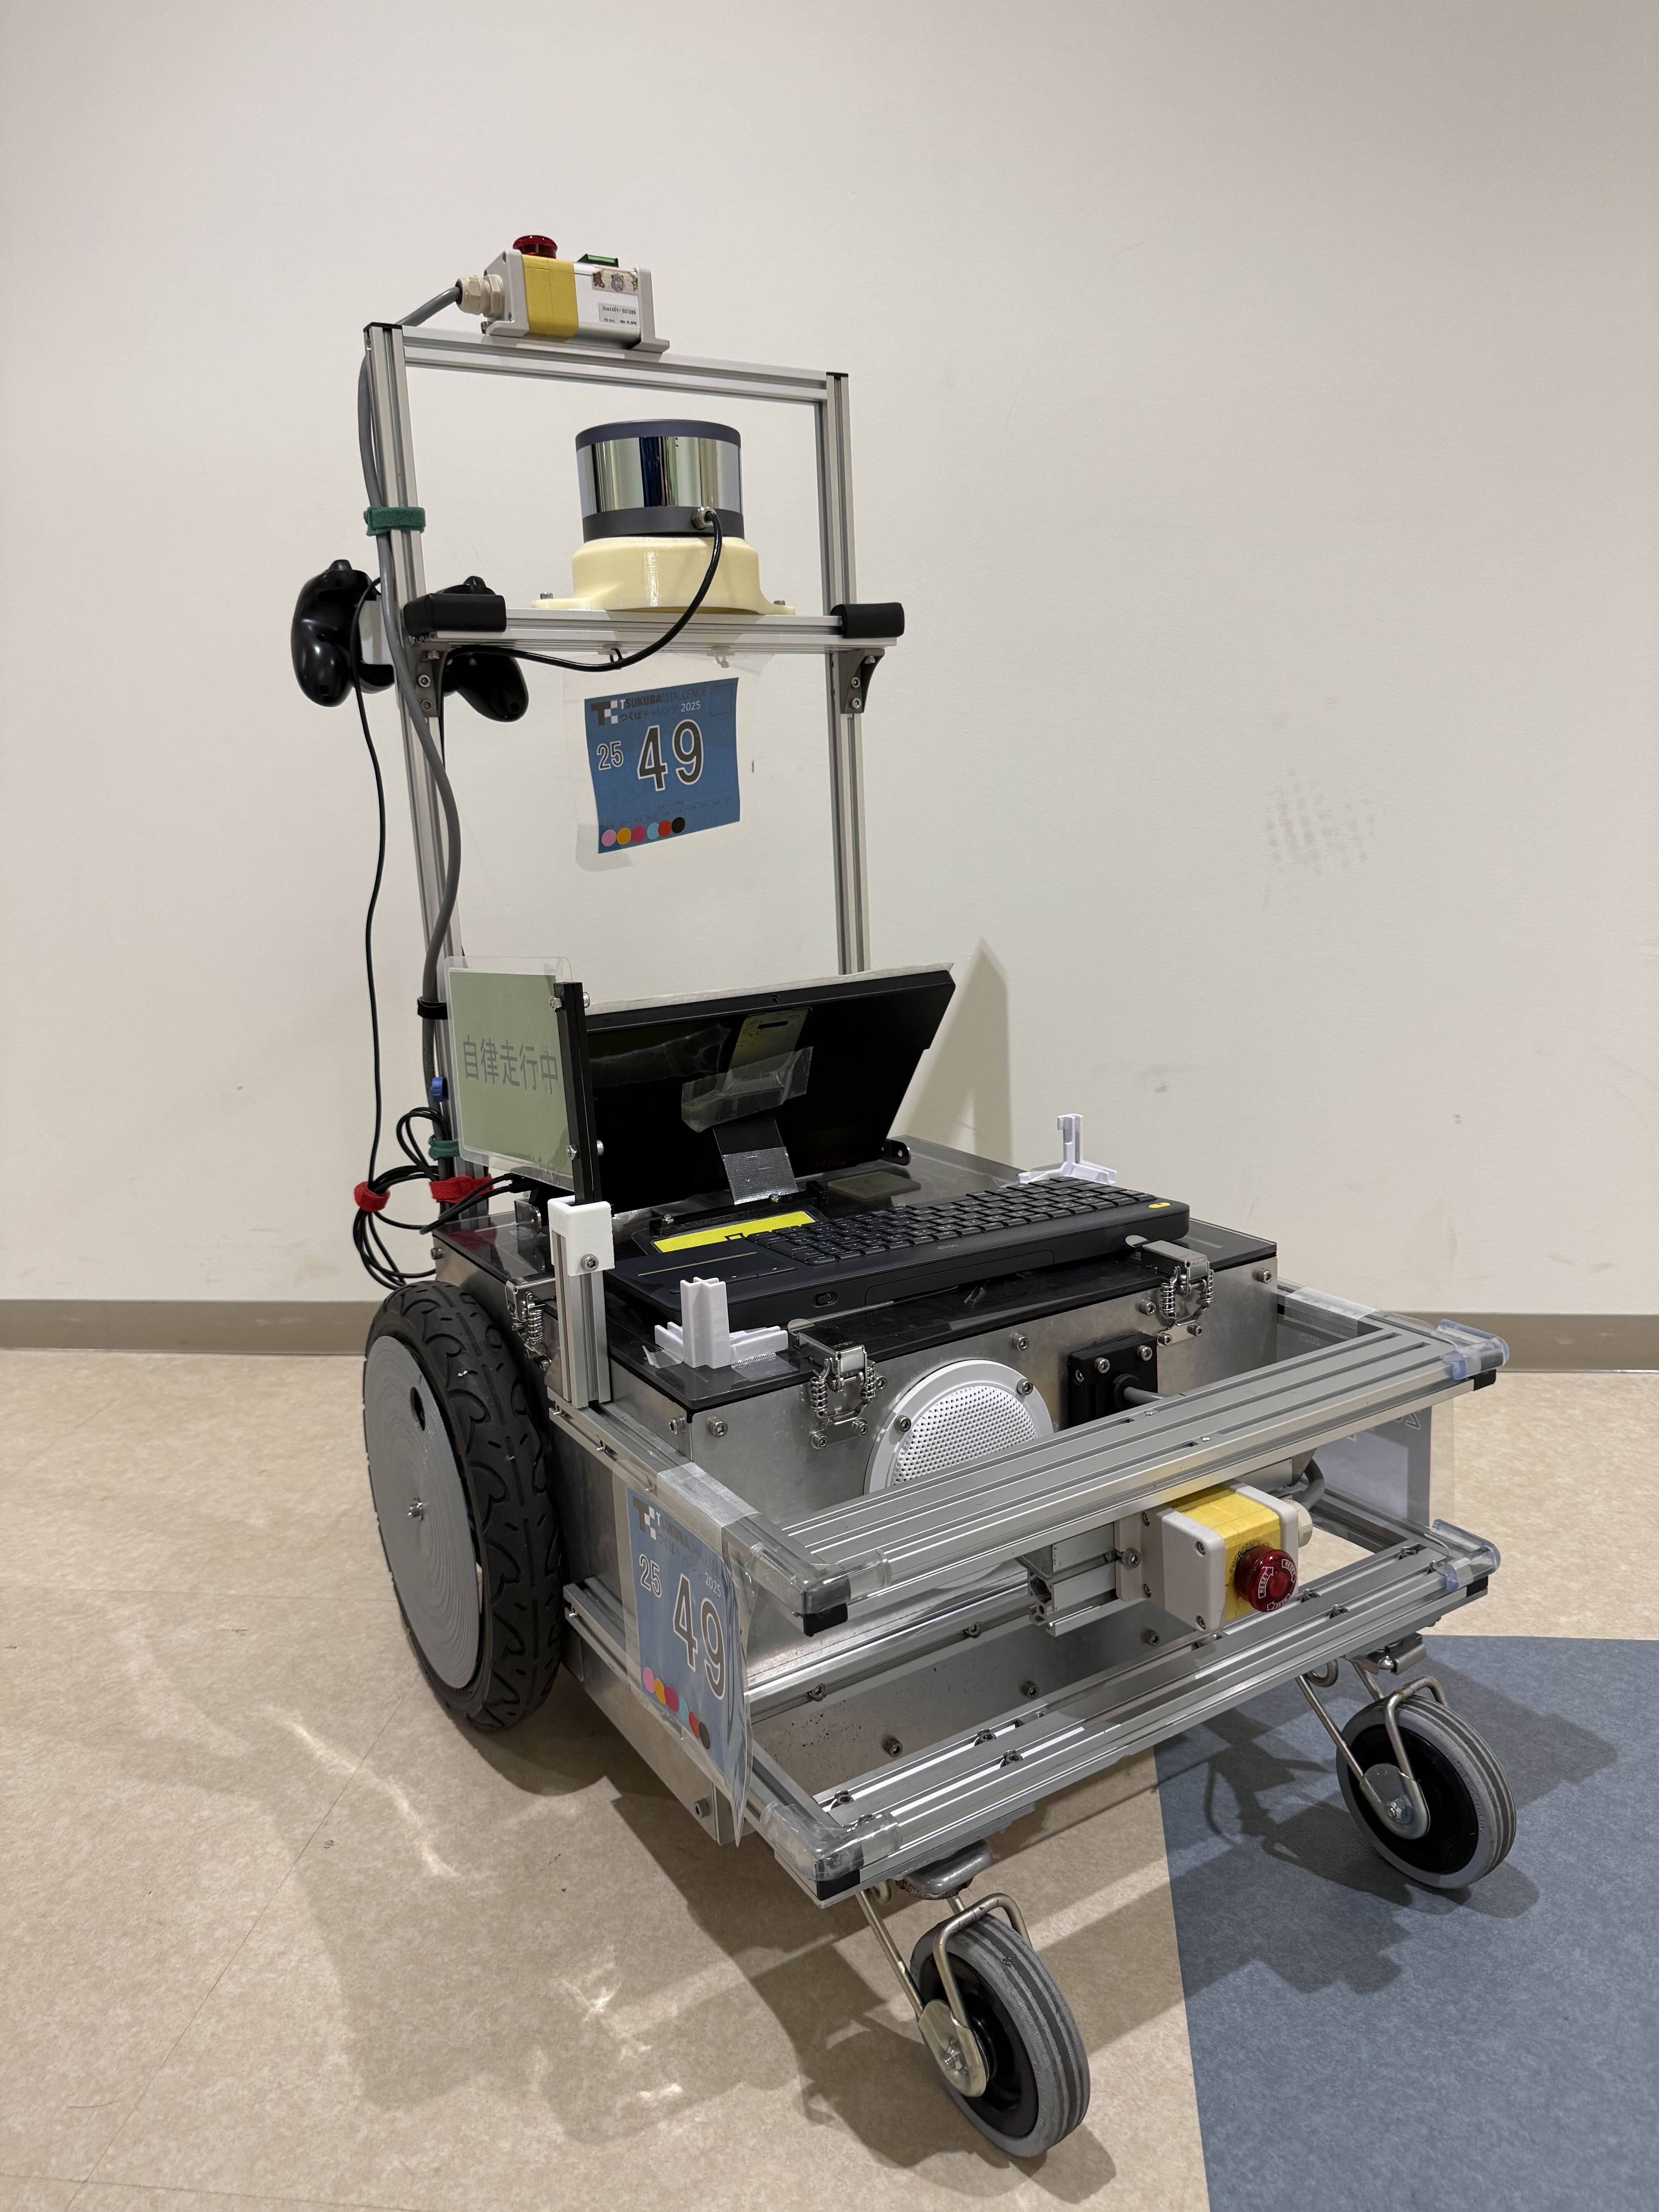
\includegraphics[keepaspectratio, scale=0.3]
      {images/orne-box3.png}
 \caption{ORNE-box3(source: \cite{井口颯人2023屋外自律移動ロボットプラットフォーム-orne})}
 \label{Fig:ORNE-box3}
\end{figure}
\begin{figure}[hbtp]
  \centering
 \includegraphics[keepaspectratio, scale=0.3]
      {images/sensor.png}
 \caption{sensor configuration}
 \label{Fig:sensor configuration}
\end{figure}
%\subsubsection{etc...}






\newpage

\section{実験結果}
%\begin{figure}[hbtp]
  %\centering
 %\includegraphics[keepaspectratio, scale=0.8]
      %{images/RaspberryPiMouse.png}
 %\caption{Example}
 %\label{Fig:Example}
%\end{figure}
\subsection{実験結果(emcl2)}
\subsubsection{実験結果(num\_particles)}
\begin{table}[H]
  \centering
  \caption{パーティクル数の違いによるゴール到達可否}
  \label{tab:num_particles_result}
  \begin{tabular}{c|c|c|c}
    \hline
    number of times & 200 & 500 (base) & 1000 \\
    \hline
    1  & $\times$ & ○ & ○ \\
    2  & ○ & ○ & $\times$ \\
    3  & $\times$ & $\times$ & $\times$ \\
    4  & ○ & ○ & ○ \\
    5  & ○ & ○ & $\times$ \\
    6  & $\times$ & $\times$ & $\times$ \\
    7  & ○ & ○ & ○ \\
    8  & ○ & ○ & ○ \\
    9  & ○ & ○ & ○ \\
    10 & ○ & ○ & ○ \\
    \hline
  \end{tabular}
\end{table}


\subsubsection{実験結果(odom\_fw\_dev\_per\_fw)}


\subsection{実験結果(Nav2\_controller)}

\subsection{実験結果(Nav2\_Costmap)}

\subsection{実験結果(Nav2\_Velocity Smoother)}

\subsection{実験結果(Nav2\_planner goal)}


%\subsubsection{etc...}

\chapter{結論}

\label{chap:conclusion}

%!TEX root = ../thesis.tex

\section{まとめ}
%\subsection{Navigation2}
%\subsection{emcl2}
%\section{論文の構成}
\begin{figure}[hbtp]
  \centering
 %\includegraphics[keepaspectratio, scale=0.8]
      %{images/RaspberryPiMouse.png}
 %\caption{Example}
 %\label{Fig:Example}
\end{figure}

\subsection{emcl2 パラメータ調整に関する総括}

本研究では,emcl2 における自己位置推定性能がロボットの走行挙動に
与える影響を明らかにするため,
オドメトリ誤差モデルおよびレーザ尤度モデルに関する
複数のパラメータを変更し,その挙動を比較・評価した.

まず,前進量に比例するオドメトリ誤差を表す
fw\_dev\_per\_fw の実験では,
値を大きくするにつれてロボットの位置推定誤差が累積し,
直進走行時に進行方向から徐々にずれていく挙動が確認された.
特に 0.5 の場合にはゴールに到達できず,
自己位置推定においてオドメトリ誤差の影響が支配的になることが
示された.一方で,0.4 以下ではゴール可能であり,
適切な範囲での設定が重要であることが分かった.

fw\_dev\_per\_rot に関する実験では,
すべての設定値においてゴール到達が可能であった.
値を大きくした場合には位置のずれが確認されたものの,
ナビゲーション全体への致命的な影響は見られず,
回転時の前進誤差は比較的ロバストであることが示唆された.

次に,前進量に比例する回転誤差を表す
rot\_dev\_per\_fw の実験では,
値を大きくしてもロボットはゴールまで到達可能であったが,
直進区間においてロボットの姿勢が徐々にずれていく傾向が確認された.
特に,高い設定値では進行方向が基準値よりも小さくなり,
姿勢推定精度の低下が見られた.

回転量に比例する回転誤差を表す
rot\_dev\_per\_rot の実験では,
値を大きくすることでレーザセンサを重視した自己位置推定となり,
ロボットの挙動が不安定になる傾向が確認された.
特に曲線走行時には,
ゴール付近で停止する事例が観測され,
過度なセンサ重視はナビゲーション性能を低下させる可能性が示された.

レーザ尤度モデルに関する実験では,
laser\_likelihood\_max\_dist を大きく設定すると,
レーザスキャンの評価が必要な場面や,
スキャン対象物が多い環境において,
ロボットが一時的に停止する挙動が確認された.
一方で,0.5 程度までの設定では,
安定した走行が可能であることが分かった.

また,range\_threshold の実験では,
基準値では近距離のスキャンを用いた安定した自己位置推定が行われていたが,
値を大きくすると遠距離のスキャンを用いるため,
位置および姿勢推定にずれが生じる場合があった.
しかし,0.5 程度までであれば,
安定性を保ったままナビゲーションを行うことが可能であった.

以上の結果より,emcl2 における各パラメータは,
オドメトリ情報とレーザセンサ情報の信頼度のバランスを調整する役割を持ち,
設定値によって自己位置推定の特性および
ロボットの走行挙動が大きく変化することが明らかとなった.
そのため,実環境におけるナビゲーションでは,
各パラメータの意味を理解した上で,
環境特性に応じた適切な調整が重要であるといえる.


\subsubsection{etc...}
\newpage

%% Back Matter
\backmatter{}
%
\chapter{実験3}

\label{chap:experiment2}

%!TEX root = ../thesis.tex

\section{実験概要}
これまでの Controller および Velocity Smoother に関する実験において,
各パラメータの上限値を増加させた場合でも,
ロボットの並進速度が一定値以上に増加しない挙動が確認された.
特に,Velocity Smoother における
\texttt{max\_velocity} や,
Controller における
\texttt{max\_vel\_x},
\texttt{max\_speed\_xy}
の値を大きく設定した場合でも,
実際の走行速度は基準値付近に制限されていた.

\begin{figure}[H]
  \centering
 \includegraphics[keepaspectratio, scale=0.6]
      {images/mvx1.0sokudo.png}
 \caption{Robot speed with max\_vel\_x = 1.0
}
 \label{Fig:Robot speed with max_vel_x = 1.0}
\end{figure}

\begin{figure}[H]
  \centering
 \includegraphics[keepaspectratio, scale=0.6]
      {images/msxy1.5sokudo.png}
 \caption{Robot speed with max\_speed\_xy = 1.5
}
 \label{Fig:Robot speed with max_speed_xy = 1.5}
\end{figure}

\begin{figure}[H]
  \centering
 \includegraphics[keepaspectratio, scale=0.6]
      {images/mvx1.2sokudo.png}
 \caption{Robot speed with max\_velocity\_x = 1.2
}
 \label{Fig:Robot speed with max_velocity_x = 1.2}
\end{figure}

この結果から,Navigation2 におけるロボットの並進速度は,
単一のパラメータによって決定されるのではなく,
Controller と Velocity Smoother の複数の速度制限パラメータが
相互に影響し合うことで制約されている可能性が示唆された.

そこで,速度制限に関与するパラメータ間の関係性を明らかにするため,
Controller の \texttt{max\_vel\_x} および \texttt{max\_speed\_xy},
ならびに Velocity Smoother の
\texttt{max\_velocity} を対象として,
それぞれの値を変化させた際のロボットの挙動を比較・評価する
追加実験を行った.

\section{実験方法}
本実験では,
Controller の \texttt{max\_vel\_x} を 1.5 に固定し,
\texttt{max\_speed\_xy} および
Velocity Smoother の速度制限パラメータ\texttt{max\_velocity\_x}を段階的に変更することで,
実際の走行速度およびロボットの挙動への影響を調査した.

Controller および Velocity Smoother における速度制限パラメータの関係性を明らかにするため,
Controller の \texttt{max\_vel\_x} を 1.5 に固定し,
\texttt{max\_speed\_xy} および
Velocity Smoother の \texttt{max\_velocity}(x成分)を
それぞれ 1.5 に設定した組み合わせ実験を行った。
本実験では,以下の 3 通りの組み合わせについて評価を行った.

\begin{itemize}
  \item \texttt{max\_vel\_x = 1.5} と \texttt{max\_speed\_xy = 1.5}
  \item \texttt{max\_vel\_x = 1.5} と \texttt{max\_velocity\_x = 1.5}
  \item \texttt{max\_vel\_x = 1.5},\texttt{max\_velocity\_x = 1.5},
        \texttt{max\_speed\_xy = 1.5}
\end{itemize}


\section{実験結果}
\begin{figure}[H]
  \centering
 \includegraphics[keepaspectratio, scale=0.6]
      {images/mvxmsxy1.5.png}
 \caption{Robot speed with max\_speed\_xy = 1.5
}
 \label{Fig:Robot speed with max_speed_xy = 1.5}
\end{figure}

\begin{figure}[H]
  \centering
 \includegraphics[keepaspectratio, scale=0.6]
      {images/mvxmvx1.5.png}
 \caption{Robot speed with max\_velocity\_x = 1.5
}
 \label{Fig:Robot speed with max_velocity_x = 1.5}
\end{figure}

\begin{figure}[H]
  \centering
 \includegraphics[keepaspectratio, scale=0.6]
      {images/sokudoall1.5.png}
 \caption{Robot speed with max\_velocity\_x = 1.5 and max\_speed\_xy = 1.5
}
 \label{Fig:Robot speed with max_velocity_x = 1.5 and max_speed_xy = 1.5}
\end{figure}

次にロボットの挙動は下のグラフに示す.\texttt{max\_vel\_x}の値は1.5とする.

% \begin{figure}[H]
%   \centering
%  \includegraphics[keepaspectratio, scale=0.6]
%       {images/s1muki.png}
%  \caption{Robot orientation with max\_speed\_xy = 1.5}
%  \label{Fig:Robot orientation with max_speed_xy = 1.5 }
% \end{figure}
\begin{figure}[H]
  \centering
 \includegraphics[keepaspectratio, scale=0.6]
      {images/s1iti2.png}
 \caption{Trajectory of the robot with max\_speed\_xy = 1.5
}
 \label{Fig:Robot position with max_speed_xy = 1.5}
\end{figure}

% \begin{figure}[H]
%   \centering
%  \includegraphics[keepaspectratio, scale=0.6]
%       {images/s2muki.png}
%  \caption{Robot orientation with max\_velocity\_x = 1.5}
%  \label{Fig:Robot orientation with max_velocity_x = 1.5 }
% \end{figure}
\begin{figure}[H]
  \centering
 \includegraphics[keepaspectratio, scale=0.6]
      {images/s2iti2.png}
 \caption{Trajectory of the robot with max\_velocity\_x = 1.5
}
 \label{Fig:Robot position with max_velocity_x = 1.5}
\end{figure}

% \begin{figure}[H]
%   \centering
%  \includegraphics[keepaspectratio, scale=0.6]
%       {images/s3muki.png}
%  \caption{Robot orientation with max\_velocity\_x = 1.5 and max\_speed\_xy = 1.5}
%  \label{Fig:Robot orientation with max_velocity_x = 1.5 and max_speed_xy = 1.5}
% \end{figure}
\begin{figure}[H]
  \centering
 \includegraphics[keepaspectratio, scale=0.6]
      {images/s3iti2.png}
 \caption{Trajectory of the robot with max\_velocity\_x = 1.5 and max\_speed\_xy = 1.5
}
 \label{Fig:Robot position with max_velocity_x = 1.5 and max_speed_xy = 1.5}
\end{figure}


\begin{table}[H]
  \centering
  \caption{Experimental Results for Speed Limitation Parameter Combinations}
  \label{tab:speed_param_combination}
  \begin{tabular}{|l|c|l|}
    \hline
    Increased parameters & Speed change & Goal achievement \\ \hline
    All three parameters &
    Significant increase &
    Unstable, goal not achieved \\ \hline
    max\_vel\_x, max\_velocity\_x &
    Moderate increase &
    Stable, goal achieved \\ \hline
    max\_vel\_x, max\_speed\_xy &
    No increase &
    Stable, goal achieved \\ \hline
  \end{tabular}
\end{table}

%\subsection{速度制限パラメータの組み合わせによる影響}

% Controller および Velocity Smoother における速度制限パラメータの関係性を明らかにするため,
% Controller の \texttt{max\_vel\_x} を 1.5 に固定し,
% \texttt{max\_speed\_xy} および
% Velocity Smoother の \texttt{max\_velocity}(x成分)を
% それぞれ 1.5 に設定した組み合わせ実験を行った。
% 本実験では,以下の 3 通りの組み合わせについて評価を行った.

% \begin{itemize}
%   \item \texttt{max\_vel\_x = 1.5} と \texttt{max\_speed\_xy = 1.5}
%   \item \texttt{max\_vel\_x = 1.5} と \texttt{max\_velocity\_x = 1.5}
%   \item \texttt{max\_vel\_x = 1.5},\texttt{max\_velocity\_x = 1.5},
%         \texttt{max\_speed\_xy = 1.5}
% \end{itemize}

その結果,
3 つすべてのパラメータを 1.5 に設定した場合,
最も高い並進速度が確認されたが,
走行中に経路から外れ,
コース脇の段差方向へ進行したため,
ゴールに到達することはできなかった.
このことから,
速度制限を同時に緩和しすぎると,
経路追従性や安定性が低下することが確認された.

一方,
\texttt{max\_vel\_x = 1.5} と
\texttt{max\_velocity\_x = 1.5} の組み合わせでは,
速度が基準値である 0.6 を超えて明確に上昇したにもかかわらず,
ロボットは安定した挙動を保ち,
ゴールまで到達することができた.
この結果は,
Controller と Velocity Smoother の速度上限を適切に一致させることで,
速度向上とナビゲーションの安定性を両立できる可能性を示している.

また,
\texttt{max\_vel\_x = 1.5} と
\texttt{max\_speed\_xy = 1.5} の組み合わせでは,
走行中の速度は基準値である 0.6 以上には増加せず,
他のパラメータによる制限が依然として有効であることが確認された.
この条件では,
最初の曲がり角付近で一時的に停止する挙動が見られたものの,
最終的にはゴールに到達しており,
ナビゲーション自体は安定していた.

以上の結果から,
Navigation2 における実際の走行速度は,
単一の速度制限パラメータではなく,
Controller と Velocity Smoother にまたがる複数の制約条件の
組み合わせによって決定されることが明らかとなった.
特に,
すべての制限を同時に緩和すると速度は向上するが,
経路追従性能が低下する一方で,
一部の制限のみを調整することで,
安定性を保ったまま速度向上が可能であることが示唆された.

%

\end{document}